Anhand der im vorherigen Kapitel \ref{sec:Anwendungsszenarien} genannten
Anwendungsszenarien lassen sich die einzelnen Schnittstellen zwischen den
Modulen ableiten. In \abbildung{Schnittstellen} ist ein schematischer Aufbau
der Module dargestellt. Die Schnittstellen zwischen diesen sind numerisch
gekennzeichnet.

\begin{figure}[H]
\centering
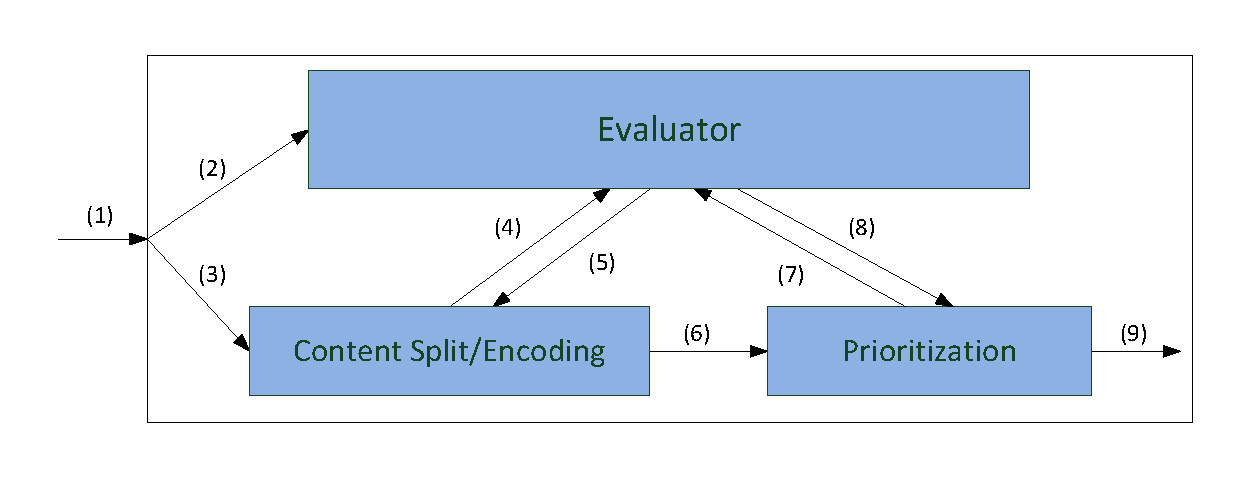
\includegraphics[width=\textwidth]{Schnittstellen.pdf}
\caption{Schnittstellen der Module}
\label{fig:Schnittstellen}
\end{figure}

Zur Vereinfachung werden der Relevanzwert, die x-Position, die
y-Position, die Länge in x-Richtung, die Länge in y-Richtung als Relevanzdaten
bezeichnet. Daraus ergeben sich die folgenden Verallgemeinerungen:

\textbf{Schnittstelle (1)}

Die Schnittstelle (1) ist die Gesamtschnittstelle. Hier wird der
Content an das Modul übergeben. Weiterhin erfolgt die Übergabe der \gls{DOID}, des
Datentyps und eines Flags, welches angibt, ob eine Zeitangabe berücksichtigt
werden soll.
Optional sind ein oder mehrere zeichengenaue Positionsangaben mit einem
Relevanzwert anzugeben. Der Relevanzwert weist hierbei eine
prozentuale Angabe im Bereich von $0$ bis $100$ auf. Dabei wird $0$ als
unwichtig und $100$ als sehr wichtig eingestuft. Die Positionsangaben beinhalten
zum einen den Startpunkt des relevanten Bereiches mit einer x- und y-Koordinate. Weiterhin
wird die Fläche des Bereiches mit einer Länge in x- und y-Richtung angegeben.
Die Angabe der Positionen und des Relevanzwertes ist beispielsweise notwendig,
wenn diese Daten nicht selbst berechnet werden sollen, sondern der Benutzer
diese über eine grafische Benutzeroberfläche vorgibt.\newline
System-Input $\rightarrow$ SenderModul: Content, \gls{DOID}, Datentyp,
Timestampflag, Relevanzdaten

\textbf{Schnittstelle (2)}

An den Evaluator wird von den Eingangsdaten der Schnittstelle (1)
der Content übergeben. Zusätzlich werden die Relevanzwerte mit den
Positionsangaben übermittelt, wenn diese vorgegeben wurden.\newline
SenderModul $\rightarrow$ Evaluator: Content, Relevanzdaten  

\textbf{Schnittstelle (3)}

Aus Schnittstelle (1) wird an die Partitionierung
die \gls{DOID}, der Datentyp, der Content und das Zeitflag
weitergegeben.\newline
SenderModul $\rightarrow$ Split/Encoding: Content, \gls{DOID}, Datentyp,
Timestampflag

\textbf{Schnittstelle (4)}

Damit der Evaluator nachvollziehen kann, welches Datenpaket gerade bearbeitet
wird, erfolgt die Übergabe der \gls{DOID} und des Datentyps. \newline
Split/Encoding $\rightarrow$ Evaluator: \gls{DOID}, Datentyp

\textbf{Schnittstelle (5)}

Als Antwort auf die eingehenden Daten der Schnittstelle (4)
erfolgt die Rückgabe der relevanten Bereiche mit den Positionen und den
dazugehörigen Relevanzwerten durch den Evaluator. \newline
Evaluator $\rightarrow$ Split/Encoding: Relevanzdaten   

\textbf{Schnittstelle (6)}

Nach der Zerlegung der Blöcke werden die einzelnen
Datenblöcke mit den dazugehörigen Datenblockheadern an die
Priorisierung übergeben. \newline
Split/Encoding $\rightarrow$ Prioritization: Datenblock

\textbf{Schnittstelle (7)}

Durch Übergabe der \gls{DOID}, des Datentypes und der Positionsangaben kann der
Content identifiziert werden. \newline
Prioritization $\rightarrow$ Evaluator: \gls{DOID}, Datentyp, Relevanzdaten

\textbf{Schnittstelle (8)}

Durch Erhalt der Daten in Schnittstelle (7) kann für
den Datenblock eine Priorität berechnet werden, welche an die Priorisierung übergeben
wird. Die Priorität wird als reelle Zahl aufgefasst und ist ähnlich dem
Relevanzwert eine prozentuale Größe zwischen $0$ und $100$. \newline
Evaluator $\rightarrow$ Prioritization: Prioritätswert

\textbf{Schnittstelle (9)}

Nach der Priorisierung werden die priorisierten Datenblöcke mit den
Datenblockheadern und der Priorität an das Verpackungsmodul übergeben. \newline
Prioritization $\rightarrow$ Packetizer: Datenblock

Bei den Schnittstellen ist zu beachten, dass manche Angaben abhängig von den
jeweiligen Datentypen sind und für den Fall nicht benutzt oder
standardmäßig auf einen bestimmten Wert gesetzt werden. Beispielsweise benötigt
ein Text als Positionsangaben keine Länge in y-Richtung. Diese ist bei einem
Bild jedoch zwingend notwendig. Die nachfolgende Tabelle
\ref{tab:RelevanzDatenBelegung} stellt die Verwendung der Relevanzdaten bei
verschiedenen Datentypen noch einmal übersichtlich dar. Dabei sind die
Positions- und Längenangaben bei einem Text zeichengenau und bei einem Bild
pixelgenau. Die Positionsangabe bei einem Text ist zweidimensional. Damit ist
auf der Empfängerseite die genaue Stelle bekannt, an der das Textfragment
platziert wird.

\begin{longtable}{|l|ccc|}
\caption{{\"U}bersicht der Relevanzdaten im Bezug zum Datentyp} \\
\hline
\label{tab:RelevanzDatenBelegung}
  & \textbf{Sensor} & \textbf{Text} & \textbf{Bild}\\
\hline{2-4}
  \textbf{Relevanzwert}     & x & x & x \\
  \textbf{x-Position}       & 0 & x & x \\
  \textbf{y-Position}       & 0 & x & x \\
  \textbf{Länge x-Richtung} & 0 & x & x \\
  \textbf{Länge y-Richtung} & 0 & 0 & x \\
\hline
\caption*{ 0 nicht verwendet, x verwendet }
\end{longtable}
